\documentclass[a4paper, 14pt]{extarticle}

\usepackage{../mystyle}

\begin{document}
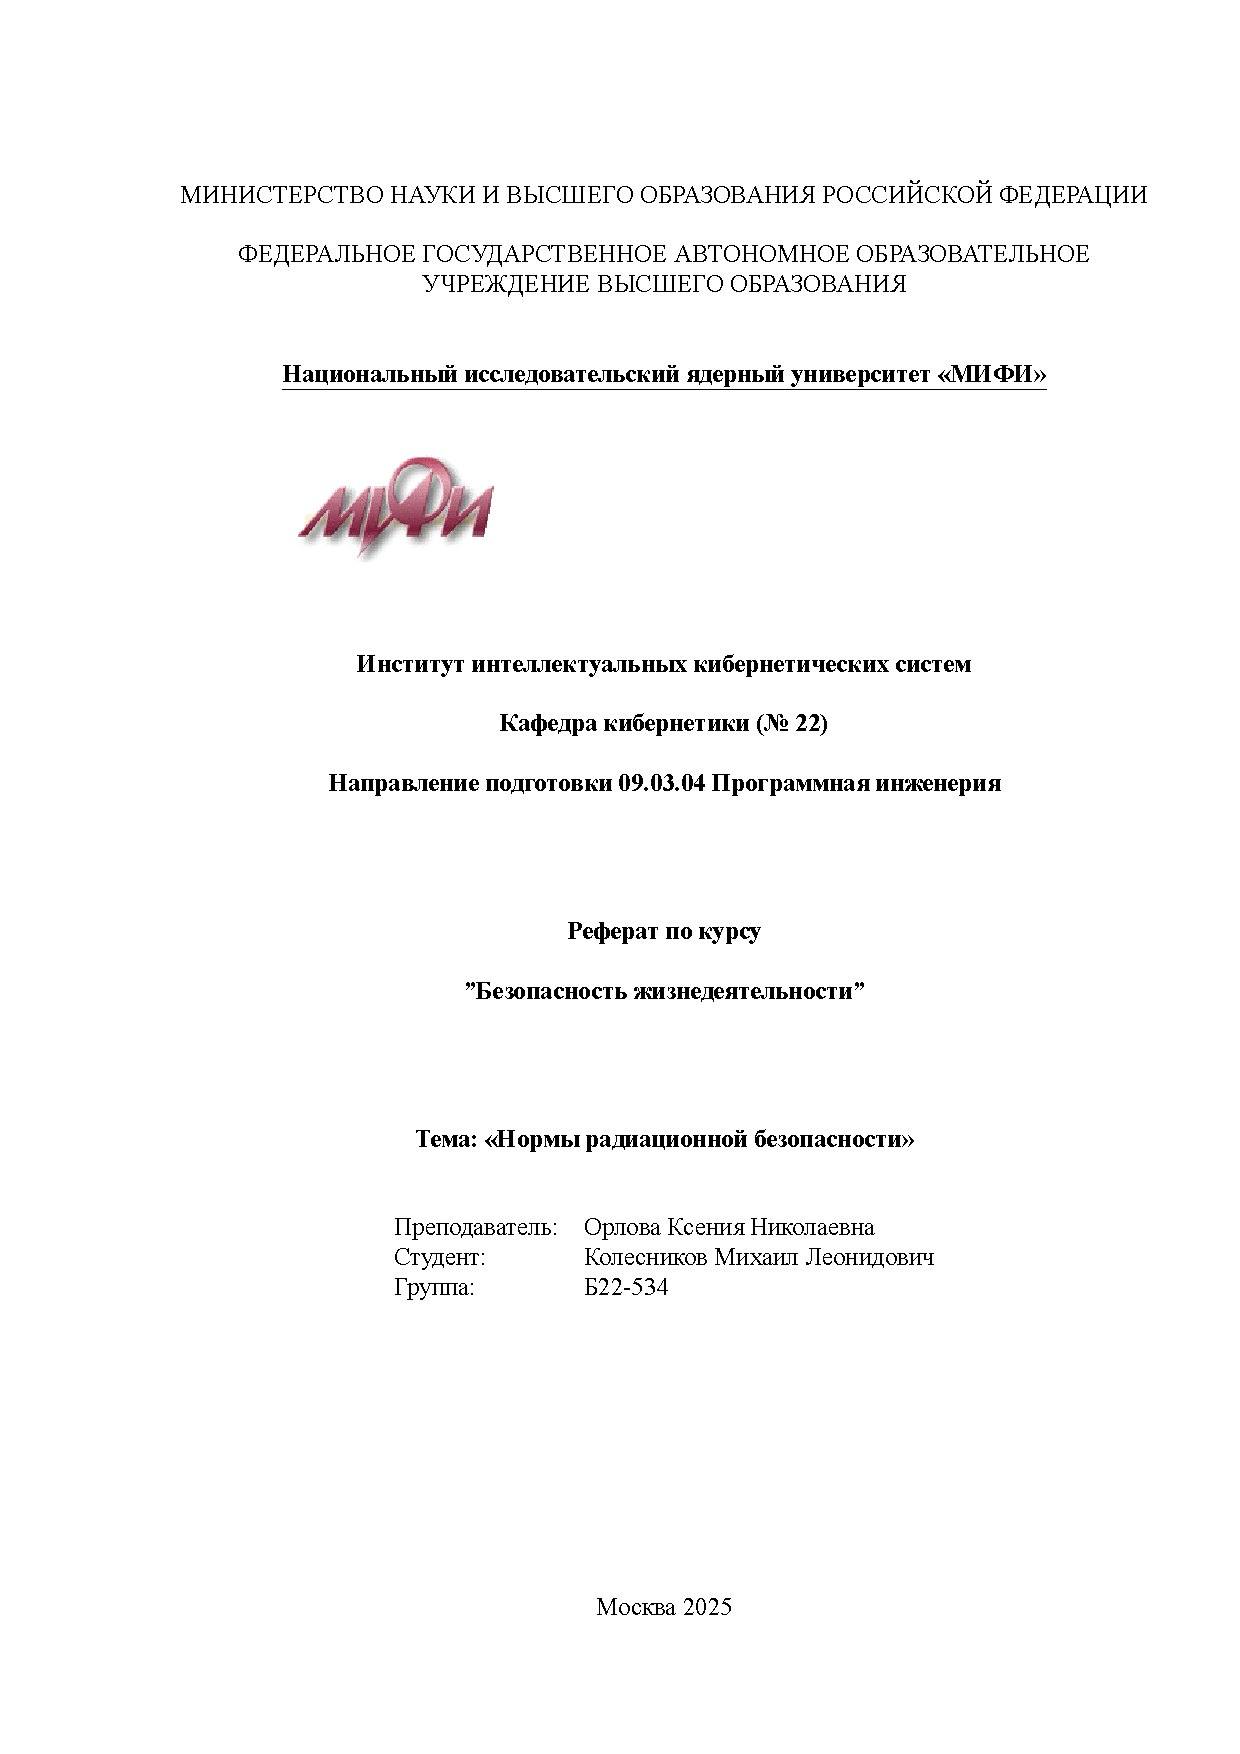
\includepdf[pages={1}]{../titul/titul.pdf}
\tableofcontents
\newpage

\section{Введение}

Радиационная безопасность остается одной из наиболее актуальных и стратегически важных проблем современности. С развитием атомной энергетики, медицины и промышленного применения радиоактивных материалов вопросы обеспечения безопасности жизнедеятельности приобретают критическое значение. Случаи радиационных инцидентов в прошлом, такие как аварии на Чернобыльской АЭС и Фукусима, продемонстрировали необходимость строгого регулирования использования радиоактивных веществ и обеспечения защиты населения, работников и окружающей среды \cite{4}.

Актуальность темы обусловлена многими факторами:

\begin{itemize}
    \item \textbf{Расширение применения радиационных технологий.} От диагностики и лечения заболеваний до промышленных процессов и энергетики — радиационные технологии находят применение в различных секторах, что требует универсальных и строгих норм безопасности.

    \item \textbf{Глобализация и международная интеграция.} Разные страны и международные организации разрабатывают собственные стандарты, что создает необходимость их анализа, сравнения и возможной гармонизации.

    \item \textbf{Эволюция научных исследований.} Новейшие исследования в области радиационной защиты, мониторинга и количественной оценки дозовых воздействий позволяют совершенствовать нормативы с целью минимизации возможного ущерба \cite{3}.
\end{itemize}

Цель данной работы — провести глубокий аналитический обзор нормативов радиационной безопасности, изучить противоречия между различными международными и национальными стандартами, критически оценить их практическое применение в различных отраслях, а также выявить тенденции в развитии нормативно-правового регулирования в данной области.

\section{Основная часть}

\subsection{Современные международные стандарты радиационной безопасности}

Международное сообщество традиционно придает большое значение разработке единых стандартов в области радиационной защиты. Международное агентство по атомной энергии (МАГАТЭ) \cite{4} и Международная комиссия по радиационной защите (МКРЗ) \cite{5} являются основными источниками рекомендаций, которые обеспечивают международное сотрудничество и обмен опытом. Эти организации разработали следующие ключевые документы:

\begin{itemize}
    \item \textbf{Основные рекомендации МКРЗ.} В документах МКРЗ определены базовые принципы радиационной защиты, такие как принцип оптимизации (ALARA), принцип индивидуальной и коллективной защиты, а также установление предельно допустимых доз. Основные принципы изложены в ряде отчетов, где уделяется внимание как профессиональной, так и общей популяции \cite{5}.

    \item \textbf{Стандарты МАГАТЭ.} Документы МАГАТЭ, например, «Safety Fundamentals» и «Safety Standards Series», представляют систематизированные нормы и критерии, обязательные для применения в странах-участницах. Эти документы охватывают все этапы работы с источниками ионного излучения — от проектирования до эксплуатации и ликвидации последствий аварий \cite{4}.

    \item \textbf{Европейская комиссия и международные конвенции.} Современные нормы, утвержденные в рамках Европейского союза, учитывают более жесткие требования к мониторингу и контролю, а также расширенный перечень мер по экстренному реагированию в случае радиационных инцидентов \cite{6}.
\end{itemize}

Важно отметить, что несмотря на общие принципы, между международными стандартами нередко наблюдаются различия, вызванные особенностями национальных систем регулирования, климатическими, демографическими и культурными факторами. Например, применение принципа оптимизации в Европе может иметь более строгие нормативные рамки по сравнению с некоторыми странами Азии, где история радиационных происшествий и уровень промышленного развития диктуют иной подход \cite{7}. Такие различия формируют основу для дальнейших сравнительных исследований.

\subsection{Российские нормативы: НПБ-99/2009 и ОСПОРБ-99/2010 с критическим анализом}

В Российской Федерации нормативно-правовая база в области радиационной безопасности представлена комплексом документов, включающих Нормы физико-химической безопасности (НПБ-99/2009) и Общероссийский стандарт по обеспечению радиационной безопасности (ОСПОРБ-99/2010) \cite{8}.

\subsubsection{НПБ-99/2009}

НПБ-99/2009 устанавливают предельно допустимые концентрации радиоактивных веществ в различных средах, а также лимиты облучения для работников и населения. Одной из положительных сторон данного нормативного акта является его широкая применимость в разных отраслях: от ядерной энергетики до медицины. Однако критический анализ выявляет следующие проблемы:

\begin{itemize}
    \item \textbf{Несовместимость с международными стандартами.} Несмотря на попытки интеграции международного опыта, в некоторых пунктах нормы расходятся с рекомендациями МАГАТЭ и МКРЗ, что приводит к трудностям в межгосударственном сотрудничестве \cite{9}.

    \item \textbf{Ограниченное применение принципа оптимизации.} В документе недостаточно детально описаны требования по ALARA, что затрудняет разработку мероприятий по минимизации дозового воздействия в прикладных областях.

    \item \textbf{Отсутствие регулярного обновления.} С учетом быстрого прогресса в области исследования радиационного воздействия, нормы требуют более оперативного пересмотра и модернизации, что не всегда осуществляется своевременно \cite{10}.
\end{itemize}

\subsubsection{ОСПОРБ-99/2010}

Общероссийский стандарт по обеспечению радиационной безопасности определяет требования к организации радиационной защиты объектов различного назначения. Среди его достоинств можно отметить:

\begin{itemize}
    \item \textbf{Комплексный подход.} Документ охватывает широкий спектр вопросов: от технических мер защиты до организационных аспектов и мероприятий по ликвидации последствий аварий.

    \item \textbf{Введение системного контроля.} ОСПОРБ-99/2010 предусматривает обязательное проведение мониторинга и контроля состояния радиационной обстановки на объектах, что способствует повышению безопасности на практике \cite{8}.
\end{itemize}

Критический анализ выявляет и минусы:

\begin{itemize}
    \item \textbf{Слабая интеграция с международными рекомендациями.} Как и в случае с НПБ-99/2009, некоторые положения стандарта недостаточно соответствуют последним рекомендациям МАГАТЭ, что может создавать барьеры для обмена опытом и внедрения лучших практик.

    \item \textbf{Нечеткая граница ответственности.} В документах иногда отсутствует четкое распределение ответственности между различными ведомствами, что усложняет оперативное реагирование в кризисных ситуациях \cite{9}.
\end{itemize}

\subsection{Сравнение с нормативами других стран (ЕС, США, Япония)}

\subsubsection{Европейский Союз}

В Европейском Союзе контроль за радиационной безопасностью регламентируется рядом директив и рекомендаций, основными из которых являются:

\begin{itemize}
    \item \textbf{Директива 2013/59/Euratom.} Данная директива устанавливает общие требования для защиты от радиационных рисков, определяя предельно допустимые дозы для работников и населения, а также правила их контроля на объектах ядерной энергетики и в медицинском секторе \cite{6}.

    \item \textbf{Европейская система раннего предупреждения.} Один из примеров практического применения нормативов — создание сети мониторинга и быстрого реагирования в случае возникновения радиационных инцидентов, что значительно повышает эффективность мер защиты \cite{7}.
\end{itemize}

\subsubsection{США}

Стандарты радиационной безопасности в США разрабатываются такими организациями, как:

\begin{itemize}
    \item \textbf{Nuclear Regulatory Commission (NRC).} Основные документы NRC, включая 10 CFR Part 20, определяют требования к ограничению доз облучения для работников и населения. Особое внимание уделяется как профилактике аварий, так и разработке сценариев экстренного реагирования \cite{11}.

    \item \textbf{Environmental Protection Agency (EPA).} Документы EPA касаются вопросов радиационной защиты окружающей среды и контроля загрязнения атмосферного воздуха и водных объектов радионуклидами, что демонстрирует многоуровневый подход к проблеме \cite{12}.
\end{itemize}

\subsubsection{Япония}

После аварии на Фукусима в 2011 году Япония значительно пересмотрела свои подходы к радиационной безопасности:

\begin{itemize}
    \item \textbf{Ужесточение норм для аварийных ситуаций.} Новые нормативы предусматривают более жесткие ограничения и меры по защите населения в экстренных ситуациях.

    \item \textbf{Разработка системы многоуровневой защиты.} Внедрение комплексного мониторинга, охватывающего как промышленные объекты, так и населенные пункты, позволило снизить потенциальные риски для здоровья \cite{13}.
\end{itemize}

Сравнительный анализ показывает, что, несмотря на общие принципы международной радиационной безопасности, нормативные документы разных стран имеют свои специфические особенности, продиктованные историческим опытом, уровнем технологического развития и уровнем подготовки специалистов. Наиболее значимым является то, что международные документы и стандарты позволяют создать базу для унификации требований, однако локальные особенности приводят к ряду противоречий, которые требуют дальнейшего согласования на уровне международного права \cite{6,11}.

\subsection{Практические аспекты применения норм на разных объектах}

Применение норм радиационной безопасности на практике требует адаптации установленных требований к условиям различных отраслей:

\subsubsection{Медицина}

В медицине радиационные технологии широко применяются в диагностике (рентгеновские исследования, компьютерная томография) и в терапии (лучевая терапия онкологических заболеваний). Практика показывает, что:

\begin{itemize}
    \item \textbf{Соблюдение дозовых лимитов.} Работники и пациенты должны строго контролироваться, используя специальное оборудование для дозиметрического контроля. Например, современные цифровые дозиметры позволяют оперативно отслеживать уровень облучения и принимать корректирующие меры \cite{14}.

    \item \textbf{Повышение квалификации персонала.} Необходим регулярный тренинг специалистов по радиационной безопасности, что помогает минимизировать вероятность ошибок при использовании оборудования \cite{14}.

    \item \textbf{Разработка стандартных операционных процедур (СОП).} На основании международных и национальных стандартов разработаны СОП, которые регламентируют проведение процедур с использованием ионизирующего излучения.
\end{itemize}

\subsubsection{Энергетика}

В атомной энергетике применение норм радиационной безопасности является жизненно важным:

\begin{itemize}
    \item \textbf{Мониторинг состояния оборудования.} Современные АЭС оснащаются системами онлайн-мониторинга, что позволяет в режиме реального времени отслеживать параметры радиационной обстановки и предотвращать аварийные ситуации \cite{15}.

    \item \textbf{Планирование экстренного реагирования.} Аварийные планы, разработанные на базе нормативных документов, включают схемы эвакуации, системы оповещения и меры по ликвидации последствий в случае аварии. Эти практики регулярно проходят учения и испытания.

    \item \textbf{Контроль за обращением с ядерными материалами.} Строгий режим учета и контроля радиоактивных материалов, а также их транспортировки минимизируют риски несанкционированного доступа и возможных злоупотреблений \cite{15}.
\end{itemize}

\subsubsection{Промышленность}

Промышленное использование радиоактивных источников требует уникального подхода к радиационной защите:

\begin{itemize}
    \item \textbf{Обеспечение безопасности персонала.} На предприятиях применяются индивидуальные средства защиты, зоны контроля и специальные помещения для хранения радиоактивных материалов. Регулярное проведение оценок рисков помогает выявлять потенциальные угрозы.

    \item \textbf{Контроль и сертификация оборудования.} Современная промышленность обязана проводить периодическую проверку и сертификацию оборудования, использующего источники ионизирующего излучения.

    \item \textbf{Интеграция автоматизированных систем мониторинга.} Разработка систем автоматического мониторинга позволяет своевременно выявлять любые отклонения от нормативных показателей, что является важным элементом обеспечения безопасности \cite{12}.
\end{itemize}

\subsection{Новейшие исследования в области радиационной защиты}

Научно-исследовательский сектор активно занимается вопросами оптимизации нормативов радиационной безопасности. Современные исследования направлены на:

\begin{itemize}
    \item \textbf{Разработку новых методов дозиметрии.} Применение инновационных материалов и сенсоров позволяет повысить точность измерения уровня облучения, что ведет к более корректной оценке риска.

    \item \textbf{Анализ биологических эффектов низких доз радиации.} Современные биомедицинские исследования помогают лучше понять долгосрочные последствия воздействия и определить пороговые значения, которые должны быть учтены в нормативных документах \cite{16}.

    \item \textbf{Моделирование распространения радиационных полей.} С помощью компьютерного моделирования разрабатываются сценарии поведения радиационных загрязнений в случае аварий, что позволяет оптимизировать системы экстренного реагирования \cite{3}.

    \item \textbf{Интердисциплинарный подход.} В современных исследованиях используются методы статистического анализа, больших данных и моделирования, что способствует более комплексной оценке риска и совершенствованию нормативных положений.
\end{itemize}

Особо следует отметить, что новые подходы часто требуют переосмысления существующих стандартов. Например, исследования, проведенные в ряде международных научных центров, показали, что действующие ограничения могут быть пересмотрены с учетом реальных биологических эффектов и новых данных о дозовой зависимости риска развития онкологических заболеваний \cite{16}. Эти результаты могут стать основой для разработки новых рекомендаций, как на уровне МАГАТЭ, так и на национальном уровне.

\subsection{Статистика радиационных инцидентов и их анализ}

Анализ статистических данных по радиационным инцидентам позволяет выявлять закономерности и слабые места в существующих системах защиты. Основные выводы, основанные на данных международных организаций и национальных агентств:

\begin{itemize}
    \item \textbf{Снижение числа крупных аварий.} За последние десятилетия наблюдается заметное снижение числа аварий на АЭС, что напрямую связано с внедрением более строгих мер безопасности и совершенствованием нормативно-правового регулирования \cite{2,4}.

    \item \textbf{Рост мелких инцидентов.} Однако статистика показывает, что количество мелких аварий и нарушений, связанных с промышленными и медицинскими источниками, остается значительным. Часто причиной становится человеческий фактор и недостаточная квалификация персонала.

    \item \textbf{Различия в отчетности.} Сравнение данных между странами выявляет существенные различия в методах учета и отчетности, что затрудняет единое понимание общей картины. В странах с развитой системой мониторинга и прозрачной отчетностью (например, в странах ЕС и США) данные являются более полными и достоверными, что позволяет оперативно реагировать на риски \cite{11,12}.
\end{itemize}

Для иллюстрации можно привести таблицу (Таблица 1), в которой приведены показатели частоты радиационных инцидентов в различных регионах. Такие сравнительные таблицы помогают выявлять наиболее уязвимые сектора и оценивать эффективность принятых мер радиационной защиты.

\begin{table}[h]
    \centering
    \caption{Сравнение статистики радиационных инцидентов (условные единицы)}
    \begin{tabular}{|l|c|c|}
        \hline
        Регион & Кол-во крупных аварий за 20 лет & Кол-во мелких инцидентов за год \\
        \hline
        ЕС     & 1-2                             & 15-20                           \\
        США    & 1-3                             & 10-15                           \\
        Япония & 2                               & 20-25                           \\
        Россия & 1-2                             & 18-22                           \\
        \hline
    \end{tabular}
\end{table}

Анализ данных показывает, что система контроля и мониторинга является ключевым фактором в предотвращении серьезных аварий. В странах с более жесткими требованиями и прозрачной отчетностью, таких как страны ЕС, наблюдаются более оперативные меры реагирования и минимизация последствий аварий \cite{7}.

\subsection{Сравнительный анализ норм радиационной безопасности в разные временные периоды}

Эволюция нормативных требований к радиационной безопасности отражает развитие технологий и накопление научных знаний. При сравнении норм, действующих в 1980--1990-х годах, и современных стандартов можно выделить следующие тенденции:

\begin{itemize}
    \item \textbf{Ужесточение предельных доз.} Современные нормативы предусматривают более низкие предельные дозы для работников и населения, что обусловлено новыми данными о биологических эффектах даже низкоинтенсивного облучения \cite{5,16}.

    \item \textbf{Расширение перечня мер защиты.} В современных нормах особое внимание уделяется не только мониторингу, но и интеграции мер по эвакуации, оперативному информированию и медицинскому сопровождению пострадавших.

    \item \textbf{Международная гармонизация нормативов.} После катастрофических инцидентов в сфере ядерной энергетики наблюдается стремление к унификации стандартов на международном уровне, что обеспечило создание общих принципов и мер контроля \cite{4,7}.

    \item \textbf{Инновационные технологии.} Внедрение цифровых систем мониторинга, автоматизированного управления и анализа больших данных позволило существенно повысить точность контроля радиационной обстановки, что нашло отражение в новых нормативных актах.
\end{itemize}

Критический анализ показывает, что хотя современные нормативы стали более комплексными и строгими, остается проблема адаптации установленных мер к специфике отдельных отраслей и региональных особенностей. Например, в условиях чрезвычайных ситуаций стандарты в странах с высокими сейсмическими рисками, как Япония, могут отличаться от российских нормативов, что требует постоянного обмена опытом и доработки национальных документов \cite{13}.

\section{Заключение}

В ходе анализа норм радиационной безопасности можно сделать следующие выводы:

\begin{enumerate}
    \item \textbf{Актуальность и комплексность проблемы.} Современные вызовы в области применения радиационных технологий требуют интегрированного подхода, включающего как международные стандарты, так и национальные нормативы.

    \item \textbf{Неоднозначность и противоречия в нормативно-правовой базе.} Сравнительный анализ международных и российских стандартов выявил существенные различия в подходах, что затрудняет гармонизацию мер радиационной защиты и требует системного пересмотра существующих документов.

    \item \textbf{Практическая ориентированность нормативов.} Несмотря на наличие четких правил и рекомендаций, применение норм на практике зависит от специфики конкретных отраслей: медицина, энергетика, промышленность требуют особых методик контроля и оперативного реагирования.

    \item \textbf{Научно-технический прогресс как движущая сила изменений.} Новейшие исследования в области дозиметрии, моделирования радиационных полей и анализа биологических эффектов способствуют постоянному совершенствованию нормативов, что позволяет оперативно реагировать на выявленные недостатки.

    \item \textbf{Статистический анализ и опыт инцидентов.} Снижение числа крупных аварий подтверждает эффективность усиленных мер радиационной защиты, однако рост мелких инцидентов требует дополнительного внимания, особенно в вопросах повышения квалификации персонала и совершенствования систем контроля.
\end{enumerate}

Перспективы развития нормативов в области радиационной безопасности связаны с дальнейшей гармонизацией международных стандартов, внедрением инновационных технологий мониторинга и анализа, а также усилением межведомственного сотрудничества. Необходим обмен передовым опытом между странами, что позволит своевременно корректировать нормативные требования в условиях быстро меняющейся технологической и экологической обстановки \cite{4,11}.

\newpage
\begin{thebibliography}{99}
    \bibitem{2} Международное агентство по атомной энергии (МАГАТЭ). Safety Fundamentals. Документ МАГАТЭ, 2014.
    \bibitem{3} Иванов А. А., Петров Б. В. Новейшие подходы к оценке дозового воздействия и модернизация нормативов радиационной защиты. Журнал «Атомная безопасность», 2020, №3.
    \bibitem{4} Документы МАГАТЭ. Safety Standards Series. МАГАТЭ, 2014.
    \bibitem{5} Международная комиссия по радиационной защите (МКРЗ). Основные рекомендации по радиационной защите. Доклады МКРЗ, 2013.
    \bibitem{6} Европейская комиссия. Директива 2013/59/Euratom: Основные требования для радиационной защиты. Официальное издание ЕС, 2014.
    \bibitem{7} Смит Дж., Кларк Е. Сравнительный анализ нормативов радиационной безопасности в Европе и США. Журнал «Radiation Protection», 2018, №2.
    \bibitem{8} Министерство здравоохранения Российской Федерации. Нормы физико-химической безопасности (НПБ-99/2009). Официальный документ, 2009.
    \bibitem{9} Российский стандарт. Общероссийский стандарт по обеспечению радиационной безопасности (ОСПОРБ-99/2010). Документ, 2010.
    \bibitem{10} Морозов П. Н., Сидоров А. И. Критический анализ нормативных документов в области радиационной защиты в РФ. Известия «Энергетическая безопасность», 2015.
    \bibitem{11} Nuclear Regulatory Commission (NRC). 10 CFR Part 20. Официальный документ США, 2012.
    \bibitem{12} Environmental Protection Agency (EPA). Документы EPA по радиационной защите окружающей среды. Официальное издание США, 2013.
    \bibitem{13} Японское министерство экономики, торговли и промышленности. Новые стандарты радиационной защиты после Фукусима. Доклад, 2012.
    \bibitem{14} Кузнецов В. А., Семёнов Д. Ю. Применение нормативов радиационной защиты в медицинской диагностике и терапии. Журнал «Медицинская физика», 2019, №4.
    \bibitem{15} Петров С. К. Организация систем мониторинга на атомных электростанциях. Журнал «Энергетика и безопасность», 2017.
    \bibitem{16} Алексеева Е. В. Проблемы интерпретации биологических эффектов низких доз облучения. Журнал «Биомедицинская физика», 2021, №1.
\end{thebibliography}

\end{document}